\documentclass[]{article}
\usepackage{lmodern}
\usepackage{amssymb,amsmath}
\usepackage{ifxetex,ifluatex}
\usepackage{fixltx2e} % provides \textsubscript
\ifnum 0\ifxetex 1\fi\ifluatex 1\fi=0 % if pdftex
  \usepackage[T1]{fontenc}
  \usepackage[utf8]{inputenc}
\else % if luatex or xelatex
  \ifxetex
    \usepackage{mathspec}
  \else
    \usepackage{fontspec}
  \fi
  \defaultfontfeatures{Ligatures=TeX,Scale=MatchLowercase}
\fi
% use upquote if available, for straight quotes in verbatim environments
\IfFileExists{upquote.sty}{\usepackage{upquote}}{}
% use microtype if available
\IfFileExists{microtype.sty}{%
\usepackage{microtype}
\UseMicrotypeSet[protrusion]{basicmath} % disable protrusion for tt fonts
}{}
\usepackage[margin=1in]{geometry}
\usepackage{hyperref}
\hypersetup{unicode=true,
            pdftitle={Visualización en ggplot2},
            pdfborder={0 0 0},
            breaklinks=true}
\urlstyle{same}  % don't use monospace font for urls
\usepackage{color}
\usepackage{fancyvrb}
\newcommand{\VerbBar}{|}
\newcommand{\VERB}{\Verb[commandchars=\\\{\}]}
\DefineVerbatimEnvironment{Highlighting}{Verbatim}{commandchars=\\\{\}}
% Add ',fontsize=\small' for more characters per line
\usepackage{framed}
\definecolor{shadecolor}{RGB}{248,248,248}
\newenvironment{Shaded}{\begin{snugshade}}{\end{snugshade}}
\newcommand{\KeywordTok}[1]{\textcolor[rgb]{0.13,0.29,0.53}{\textbf{#1}}}
\newcommand{\DataTypeTok}[1]{\textcolor[rgb]{0.13,0.29,0.53}{#1}}
\newcommand{\DecValTok}[1]{\textcolor[rgb]{0.00,0.00,0.81}{#1}}
\newcommand{\BaseNTok}[1]{\textcolor[rgb]{0.00,0.00,0.81}{#1}}
\newcommand{\FloatTok}[1]{\textcolor[rgb]{0.00,0.00,0.81}{#1}}
\newcommand{\ConstantTok}[1]{\textcolor[rgb]{0.00,0.00,0.00}{#1}}
\newcommand{\CharTok}[1]{\textcolor[rgb]{0.31,0.60,0.02}{#1}}
\newcommand{\SpecialCharTok}[1]{\textcolor[rgb]{0.00,0.00,0.00}{#1}}
\newcommand{\StringTok}[1]{\textcolor[rgb]{0.31,0.60,0.02}{#1}}
\newcommand{\VerbatimStringTok}[1]{\textcolor[rgb]{0.31,0.60,0.02}{#1}}
\newcommand{\SpecialStringTok}[1]{\textcolor[rgb]{0.31,0.60,0.02}{#1}}
\newcommand{\ImportTok}[1]{#1}
\newcommand{\CommentTok}[1]{\textcolor[rgb]{0.56,0.35,0.01}{\textit{#1}}}
\newcommand{\DocumentationTok}[1]{\textcolor[rgb]{0.56,0.35,0.01}{\textbf{\textit{#1}}}}
\newcommand{\AnnotationTok}[1]{\textcolor[rgb]{0.56,0.35,0.01}{\textbf{\textit{#1}}}}
\newcommand{\CommentVarTok}[1]{\textcolor[rgb]{0.56,0.35,0.01}{\textbf{\textit{#1}}}}
\newcommand{\OtherTok}[1]{\textcolor[rgb]{0.56,0.35,0.01}{#1}}
\newcommand{\FunctionTok}[1]{\textcolor[rgb]{0.00,0.00,0.00}{#1}}
\newcommand{\VariableTok}[1]{\textcolor[rgb]{0.00,0.00,0.00}{#1}}
\newcommand{\ControlFlowTok}[1]{\textcolor[rgb]{0.13,0.29,0.53}{\textbf{#1}}}
\newcommand{\OperatorTok}[1]{\textcolor[rgb]{0.81,0.36,0.00}{\textbf{#1}}}
\newcommand{\BuiltInTok}[1]{#1}
\newcommand{\ExtensionTok}[1]{#1}
\newcommand{\PreprocessorTok}[1]{\textcolor[rgb]{0.56,0.35,0.01}{\textit{#1}}}
\newcommand{\AttributeTok}[1]{\textcolor[rgb]{0.77,0.63,0.00}{#1}}
\newcommand{\RegionMarkerTok}[1]{#1}
\newcommand{\InformationTok}[1]{\textcolor[rgb]{0.56,0.35,0.01}{\textbf{\textit{#1}}}}
\newcommand{\WarningTok}[1]{\textcolor[rgb]{0.56,0.35,0.01}{\textbf{\textit{#1}}}}
\newcommand{\AlertTok}[1]{\textcolor[rgb]{0.94,0.16,0.16}{#1}}
\newcommand{\ErrorTok}[1]{\textcolor[rgb]{0.64,0.00,0.00}{\textbf{#1}}}
\newcommand{\NormalTok}[1]{#1}
\usepackage{graphicx,grffile}
\makeatletter
\def\maxwidth{\ifdim\Gin@nat@width>\linewidth\linewidth\else\Gin@nat@width\fi}
\def\maxheight{\ifdim\Gin@nat@height>\textheight\textheight\else\Gin@nat@height\fi}
\makeatother
% Scale images if necessary, so that they will not overflow the page
% margins by default, and it is still possible to overwrite the defaults
% using explicit options in \includegraphics[width, height, ...]{}
\setkeys{Gin}{width=\maxwidth,height=\maxheight,keepaspectratio}
\IfFileExists{parskip.sty}{%
\usepackage{parskip}
}{% else
\setlength{\parindent}{0pt}
\setlength{\parskip}{6pt plus 2pt minus 1pt}
}
\setlength{\emergencystretch}{3em}  % prevent overfull lines
\providecommand{\tightlist}{%
  \setlength{\itemsep}{0pt}\setlength{\parskip}{0pt}}
\setcounter{secnumdepth}{0}
% Redefines (sub)paragraphs to behave more like sections
\ifx\paragraph\undefined\else
\let\oldparagraph\paragraph
\renewcommand{\paragraph}[1]{\oldparagraph{#1}\mbox{}}
\fi
\ifx\subparagraph\undefined\else
\let\oldsubparagraph\subparagraph
\renewcommand{\subparagraph}[1]{\oldsubparagraph{#1}\mbox{}}
\fi

%%% Use protect on footnotes to avoid problems with footnotes in titles
\let\rmarkdownfootnote\footnote%
\def\footnote{\protect\rmarkdownfootnote}

%%% Change title format to be more compact
\usepackage{titling}

% Create subtitle command for use in maketitle
\newcommand{\subtitle}[1]{
  \posttitle{
    \begin{center}\large#1\end{center}
    }
}

\setlength{\droptitle}{-2em}
  \title{Visualización en ggplot2}
  \pretitle{\vspace{\droptitle}\centering\huge}
  \posttitle{\par}
  \author{}
  \preauthor{}\postauthor{}
  \date{}
  \predate{}\postdate{}

\usepackage[
  backend=biber,
  style=alphabetic,
  sorting=ynt,
  citestyle=authoryear
  ]{biblatex}
\addbibresource{../lit/bib.bib}

\usepackage[utf8]{inputenc}
\usepackage[spanish]{babel}

%%%% Frames
\ifxetex
    \makeatletter % undo the wrong changes made by mathspec
    \let\RequirePackage\original@RequirePackage
    \let\usepackage\RequirePackage
    \makeatother
\fi

\usepackage{xcolor}
\usepackage[tikz]{bclogo}
\usepackage[framemethod=tikz]{mdframed}
\usepackage{lipsum}
\usepackage[many]{tcolorbox}

\definecolor{bgblue}{RGB}{245,243,253}
\definecolor{ttblue}{RGB}{91,194,224}
\definecolor{llred}{RGB}{255,228,225}
\definecolor{bbblack}{RGB}{0,0,0}

\mdfdefinestyle{mystyle}{%
  rightline=true,
  innerleftmargin=10,
  innerrightmargin=10,
  outerlinewidth=3pt,
  topline=false,
  rightline=true,
  bottomline=false,
  skipabove=\topsep,
  skipbelow=\topsep
}

\newtcolorbox{curiosidad}[1][]{
  breakable,
  title=#1,
  colback=white,
  colbacktitle=white,
  coltitle=black,
  fonttitle=\bfseries,
  bottomrule=0pt,
  toprule=0pt,
  leftrule=3pt,
  rightrule=3pt,
  titlerule=0pt,
  arc=0pt,
  outer arc=0pt,
  colframe=black,
}

\newtcolorbox{nota}[1][]{
  breakable,
  freelance,
  title=#1,
  colback=white,
  colbacktitle=white,
  coltitle=black,
  fonttitle=\bfseries,
  bottomrule=0pt,
  boxrule=0pt,
  colframe=white,
  overlay unbroken and first={
  \draw[red!75!black,line width=3pt]
    ([xshift=5pt]frame.north west) -- 
    (frame.north west) -- 
    (frame.south west);
  \draw[red!75!black,line width=3pt]
    ([xshift=-5pt]frame.north east) -- 
    (frame.north east) -- 
    (frame.south east);
  },
  overlay unbroken app={
  \draw[red!75!black,line width=3pt,line cap=rect]
    (frame.south west) -- 
    ([xshift=5pt]frame.south west);
  \draw[red!75!black,line width=3pt,line cap=rect]
    (frame.south east) -- 
    ([xshift=-5pt]frame.south east);
  },
  overlay middle and last={
  \draw[red!75!black,line width=3pt]
    (frame.north west) -- 
    (frame.south west);
  \draw[red!75!black,line width=3pt]
    (frame.north east) -- 
    (frame.south east);
  },
  overlay last app={
  \draw[red!75!black,line width=3pt,line cap=rect]
    (frame.south west) --
    ([xshift=5pt]frame.south west);
  \draw[red!75!black,line width=3pt,line cap=rect]
    (frame.south east) --
    ([xshift=-5pt]frame.south east);
  },
}

\begin{document}


\section{Visualización}\label{visualizacion}

La graficación es una manera eficiente de resumir, y mostrar
información. Es fundamental entender el contexto de negocio y de la
generación de los datos para tener más información con respecto a lo que
se está graficando.

Aunqu eno hay mucha teoría alrededor de gráficos estadísticos, muchos se
describen en distintos libros de texto de estadística
\parencite[][Introducción]{unwin2015}.

\textcite[][citando a John Tukey]{unwin2015} resume el propósito de la
visualización de datos en cuatro frases:

\begin{enumerate}
\def\labelenumi{\arabic{enumi}.}
\tightlist
\item
  Las gráficas son para análsisis cualitativos o descriptivos y quizá
  semi cuantitativos, nunca para análisis profundo cuantitativo (las
  tablas son mejores para esta tarea).
\item
  Las gráficas son para realizar comparaciones (en el tiempo, entre
  grupos), no para describir cantidades particulares.
\item
  Las gráficas son para impactar (visualmente, para sorprender, para
  transmitir información), pero casi nunca sirven para reflejar patrones
  escondidos en los datos.
\item
  Las gráficas deberían de reportar un análisis de datos trabajado, fino
  y cuidadoso. Jamás deben de reemplazar el análisis. Las gráficas están
  para fortalecer el análisis, no para fundamentarlo y los gráficos
  finales en un análisis deben reflejar el análisis realizado.
\end{enumerate}

Esta sección resume algunas de las funciones implementadas para
\textbf{visualizar} datos implementados en el paquete \texttt{ggplot2}
de \texttt{R}. Está fuera de la alcance de este apartado las
consideraciones estadísticas que deben de realizarse en un análisis de
datos pues el enfoque es mostrar cómo realizar esta tarea en \texttt{R}.
En la figura \ref{fig:ciclo4} podemos ver la etapa del análisis de datos
correspondiente.

\begin{figure}[h]
    \centering
    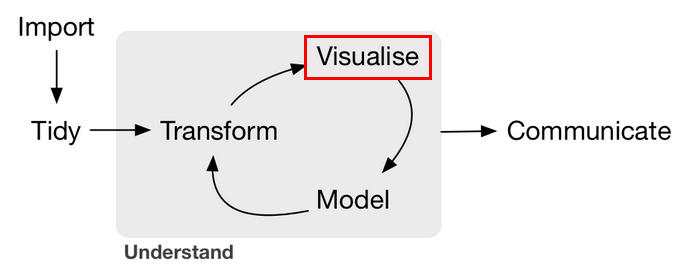
\includegraphics[width=0.75\textwidth]{../img/02_ciclo_4.png}
    \caption{Visualización en el análisis de datos \textcite[Introducción]{grolemund2016r}.}
    \label{fig:ciclo4}
\end{figure}

En \texttt{R} hay muchas maneras de realizar una tarea, esto es
particularmente cierto en lo que se refiere a visualización de datos
\parencite{basevggplot}. A fin de cuentas, lo más importante de la
visualización de datos es cuán útil es esta herramienta para el análisis
de datos y la forma en la que se le indica a la máquina como realizar la
tarea es un elemento importante solo en la medida en la que facilite el
trabajo del estadístico.

Aunque posiblemente cualquiera de los gráficos que se pueden hacer con
\texttt{ggplot2} pueden hacerse también con los gráficos implementados
en el \texttt{base\ graphics} de \texttt{R} \parencite{basevggplot},
aquí se cubre visualización en \texttt{ggplot2} principalmente debido a
que:

\begin{itemize}
\tightlist
\item
  El patrón de programación está definido formalmente mientras que en el
  \texttt{base} no lo está. Esto significa que cuando entiendes cómo
  hacer una gráfica en \texttt{ggplot2}, puedes hacer una gran cantidad
  de gráficos \parencite{basevggplot}.
\item
  \texttt{ggplot2} tiene una gran cantidad de \emph{defaults}
  predefinidos que facilitan realizar gráficos ilustrativos y estéticos
  muy rápidamente \parencite{reasonsggplot}.
\item
  \texttt{ggplot2} es compatible con
  \emph{piping}\footnote{Se introdujo el operador \textit{pipe} de \texttt{R} en la sección de transformación en este capítulo y se mencionó como ayuda en la lectura y escritura de código. Un\textit{pipeline} en programación consiste en un arreglo de elementos de procesamiento en donde la salida de cada elemento es la entrada del siguiente elemento. Este concepto fue concebido por Douglas Mcllroy \parencite{unixpipes}.}
  \parencite{notggplot}.
\item
  Muchas veces, resulta necesario realizar un mismo gráfico para varios
  subconjuntos de datos. Esta tarea se puede hacer en forma directa en
  \texttt{ggplot2} y no en el \texttt{base} a través de facetas.
\end{itemize}

Primero, se cubrirá el concepto detrás de \texttt{ggplot2}, la gramática
de las gráficas. Posteriormente, se describen los componentes de una
gráfica en \texttt{ggplot2}, las capas y sus componentes proporcionando
ejemplos en cada caso.

\subsection{La gramática de las
gráficas}\label{la-gramatica-de-las-graficas}

Es una herramienta que nos permite \parencite{wickham2010layered}:

\begin{itemize}
\tightlist
\item
  Describir los componentes de una gráfica en forma concisa
\item
  Ir más allá de los nombres de la gráfica (e.g.~scatterplot, boxplot,
  etc.)
\item
  Entender la estructura detrás de los gráficos estadísticos
\end{itemize}

\subsection{¿Qué es?}\label{que-es}

La gramática le da reglas al lenguaje y es un sistema formal para
generar enunciados \parencite{wilkinson2006grammar}.
\textcite{wilkinson2006grammar} proporciona una gramática para gráficos
que permite describir y construir una gran cantidad de gráficos
estadísticos. \parencite{wickham2010layered} implementa esta gramática
en el paquete \texttt{ggplot2} de \texttt{R} \parencite{ggplot2}.

La gramática define un gráfico estadístico como un mapeo de datos a
atributos estéticos (un color, una forma) en objetos geométricos
(barras, líneas, puntos). Además, una gráfica puede implicar
transformaciones estadísticas de los datos y se dibuja sobre un sistema
de coordenadas específico. Por último, es posible generar el mismo
gráfico en diferentes subconjuntos de los datos (facetas). La
combinación de estos factores independientes conforman un gráfico
\parencite[][p. 5]{ggplot2}.

La implementación en capas, permite que los usuarios no se limiten
únicamente a los gráficos específicos que se implementan paquete a
paquete sino que puedan realizar tantos gráficos como este lenguaje de
gráficos permita.

\subsection{Base plotting vs.~ggplot}\label{base-plotting-vs.ggplot}

Observemos una gráfica utilizando la base \texttt{diamonds} en donde
graficamos en el eje \(x\) el carataje de diamantes y en el eje \(y\) su
precio:

\begin{Shaded}
\begin{Highlighting}[]
\KeywordTok{data}\NormalTok{(diamonds, }\DataTypeTok{package =} \StringTok{"ggplot2"}\NormalTok{)}
\KeywordTok{str}\NormalTok{(diamonds)}
\end{Highlighting}
\end{Shaded}

\begin{verbatim}
## Classes 'tbl_df', 'tbl' and 'data.frame':    53940 obs. of  10 variables:
##  $ carat  : num  0.23 0.21 0.23 0.29 0.31 0.24 0.24 0.26 0.22 0.23 ...
##  $ cut    : Ord.factor w/ 5 levels "Fair"<"Good"<..: 5 4 2 4 2 3 3 3 1 3 ...
##  $ color  : Ord.factor w/ 7 levels "D"<"E"<"F"<"G"<..: 2 2 2 6 7 7 6 5 2 5 ...
##  $ clarity: Ord.factor w/ 8 levels "I1"<"SI2"<"SI1"<..: 2 3 5 4 2 6 7 3 4 5 ...
##  $ depth  : num  61.5 59.8 56.9 62.4 63.3 62.8 62.3 61.9 65.1 59.4 ...
##  $ table  : num  55 61 65 58 58 57 57 55 61 61 ...
##  $ price  : int  326 326 327 334 335 336 336 337 337 338 ...
##  $ x      : num  3.95 3.89 4.05 4.2 4.34 3.94 3.95 4.07 3.87 4 ...
##  $ y      : num  3.98 3.84 4.07 4.23 4.35 3.96 3.98 4.11 3.78 4.05 ...
##  $ z      : num  2.43 2.31 2.31 2.63 2.75 2.48 2.47 2.53 2.49 2.39 ...
\end{verbatim}

\begin{Shaded}
\begin{Highlighting}[]
\KeywordTok{plot}\NormalTok{(diamonds}\OperatorTok{$}\NormalTok{carat, diamonds}\OperatorTok{$}\NormalTok{price)}
\end{Highlighting}
\end{Shaded}

\includegraphics{ggplot2_files/figure-latex/unnamed-chunk-1-1.pdf}

Ese mismo gráfico, podemos realizarlo con la función \texttt{qplot} del
paquete\texttt{ggplot}:

\begin{Shaded}
\begin{Highlighting}[]
\KeywordTok{qplot}\NormalTok{(}\DataTypeTok{data =}\NormalTok{ diamonds, }\DataTypeTok{x =}\NormalTok{ carat, }\DataTypeTok{y =}\NormalTok{ price, }\DataTypeTok{geom =} \StringTok{"point"}\NormalTok{)}
\end{Highlighting}
\end{Shaded}

\includegraphics{ggplot2_files/figure-latex/unnamed-chunk-2-1.pdf}

En donde especificamos que la variable \texttt{carat} en la base
\texttt{diamonds} mapea al eje \(x\), la variable \texttt{price} en la
misma base al eje \(y\) y queremos que la geometría sea de puntos.

Observa que la estética de la gráfica generada con la función
\texttt{plot} es un poco distinta a la generada con \texttt{qplot}
(función que utiliza \texttt{ggplot}). Verifica la clase que tiene cada
objeto, en el primer caso no tiene y en el segundo tenemos un objeto de
clase \texttt{ggplot} que tiene atributos y que podemos guardar en un
objeto.

\subsection{ggplot}\label{ggplot}

Los componentes de la gramática de gráficas específica para
\texttt{ggplot} son:

\begin{enumerate}
\def\labelenumi{\arabic{enumi}.}
\tightlist
\item
  Una o más capas donde cada cuál tiene:

  \begin{enumerate}
  \def\labelenumii{\alph{enumii}.}
  \tightlist
  \item
    Datos
  \item
    Mapeo estético de los datos (\emph{aesthetic mappings})
  \item
    Un objeto geométrico
  \item
    Una transformación estadística
  \item
    Ajustes en las posiciones de los objetos
  \end{enumerate}
\item
  Una escala para cada estética
\item
  Un sistema de coordenadas
\item
  Una especificación de facetas
\end{enumerate}

Al graficar en \texttt{ggplot} se tiene control sobre todos estos
elementos:

\begin{Shaded}
\begin{Highlighting}[]
\KeywordTok{ggplot}\NormalTok{() }\OperatorTok{+}
\StringTok{  }\KeywordTok{layer}\NormalTok{( }\CommentTok{# una capa}
    \DataTypeTok{data =}\NormalTok{ diamonds, }\CommentTok{# datos}
    \DataTypeTok{mapping =} \KeywordTok{aes}\NormalTok{(}\DataTypeTok{x =}\NormalTok{ carat, }\DataTypeTok{y =}\NormalTok{ price), }\CommentTok{# mapeo estético}
    \DataTypeTok{geom =} \StringTok{"point"}\NormalTok{, }\CommentTok{# geometría}
    \DataTypeTok{stat =} \StringTok{"identity"}\NormalTok{, }\CommentTok{# transformación estadística}
    \DataTypeTok{position =} \StringTok{"identity"} \CommentTok{# ajuste en posición de objetos}
\NormalTok{    ) }\OperatorTok{+}\StringTok{ }
\StringTok{  }\KeywordTok{scale_y_continuous}\NormalTok{() }\OperatorTok{+}\StringTok{ }\CommentTok{# Escala para estética continua en y}
\StringTok{  }\KeywordTok{scale_x_continuous}\NormalTok{() }\OperatorTok{+}\StringTok{ }\CommentTok{# Escala para estética continua en x}
\StringTok{  }\KeywordTok{coord_cartesian}\NormalTok{() }\CommentTok{# Sistema de coordenadas}
\end{Highlighting}
\end{Shaded}

\includegraphics{ggplot2_files/figure-latex/unnamed-chunk-3-1.pdf}

\texttt{ggplot} implementa también una serie de \texttt{defaults}
\parencite[][p. 3]{ggplot2} que facilitan la escritura de nuevas
gráficas pues no es necesario especificar cada uno de los detalles al
agregar una capa. Por tanto, es posible escribir el mismo gráfico
haciendo uso de esos \texttt{defaults}:

\begin{Shaded}
\begin{Highlighting}[]
\KeywordTok{ggplot}\NormalTok{(diamonds, }\KeywordTok{aes}\NormalTok{(carat, price)) }\OperatorTok{+}\StringTok{ }\KeywordTok{geom_point}\NormalTok{()}
\end{Highlighting}
\end{Shaded}

\includegraphics{ggplot2_files/figure-latex/unnamed-chunk-4-1.pdf}

\subsection{Características
importantes}\label{caracteristicas-importantes}

Los componentes de una gráfica son ortogonales:

\begin{verbatim}
- Cambiar uno no debe romper los otros
- Una configuración distinta de componentes es válida
- Puedes construir mayor complejidad agregando capas
\end{verbatim}

\subsection{Las capas}\label{las-capas}

\texttt{ggplot} produce un objeto que se puede convertir en una gráfica.
Es decir, \texttt{R} sabe cómo convertirlo en una gráfica.

Este objeto está formado por capas, mismas que tienen sus entradas
(\emph{inputs}) particulares y que comparten argumentos del gráfico
\texttt{base} generado por la función \texttt{ggplot()}. Con el operador
\texttt{+} se van agregando las distintas capas al mismo objeto.

Así como en otros casos, el objeto en \texttt{R} puede ser guardado en
una variable, se le puede imprimir, se le puede guardar como imagen de
diferentes formatos, o se puede guardar en una lista o en un
\texttt{Rdata}.

\subsection{Componentes de una capa}\label{componentes-de-una-capa}

\subsubsection{Datos y mapa estético}\label{datos-y-mapa-estetico}

Permite mapear las columnas del \texttt{data.frame} de entrada a los
aspectos de la gráfica.

Es decir,

\begin{itemize}
\tightlist
\item
  las coordenadas \(x\), \(y\)
\item
  los grupos (definidos por otra variable)
\item
  el tamaño
\item
  el color
\item
  el relleno
\end{itemize}

Para ejemplificar, generamos una variable \(x\) que proviene de dos
distribuciones normales: mil realizaciones \(N(0, 1)\) y mil
\(N(3, 1)\). Asignamos un grupo a las primeras mil y otro a la segunda.

\begin{Shaded}
\begin{Highlighting}[]
\NormalTok{mix2norm <-}\StringTok{ }\KeywordTok{data.frame}\NormalTok{(}\DataTypeTok{x  =} \KeywordTok{c}\NormalTok{(}\KeywordTok{rnorm}\NormalTok{(}\DecValTok{1000}\NormalTok{), }\KeywordTok{rnorm}\NormalTok{(}\DecValTok{1000}\NormalTok{, }\DecValTok{3}\NormalTok{)), }
                       \DataTypeTok{grupo =} \KeywordTok{as.factor}\NormalTok{(}\KeywordTok{rep}\NormalTok{(}\KeywordTok{c}\NormalTok{(}\DecValTok{1}\NormalTok{,}\DecValTok{2}\NormalTok{),}\DataTypeTok{each=}\DecValTok{1000}\NormalTok{)))}

\KeywordTok{ggplot}\NormalTok{(mix2norm, }\KeywordTok{aes}\NormalTok{(}\DataTypeTok{x=}\NormalTok{x, }\DataTypeTok{color =}\NormalTok{ grupo)) }\OperatorTok{+}\StringTok{ }\KeywordTok{geom_density}\NormalTok{()}
\end{Highlighting}
\end{Shaded}

\includegraphics{ggplot2_files/figure-latex/unnamed-chunk-5-1.pdf}

\subsubsection{Transformaciones
estadísticas}\label{transformaciones-estadisticas}

Ésta puede ser, por ejemplo, un resumen de la entrada (\emph{input})
recibido; se especifica vía el comando \texttt{stat}. Ejemplos:

\begin{itemize}
\tightlist
\item
  binning
\item
  smoothing
\item
  boxplot
\item
  identity
\end{itemize}

Utilizamos, por ejemplo, la transformación \emph{bin}, misma que se
especifica en el objeto geométrico:

\begin{Shaded}
\begin{Highlighting}[]
\KeywordTok{ggplot}\NormalTok{(mix2norm, }\KeywordTok{aes}\NormalTok{(}\DataTypeTok{x=}\NormalTok{x, }\DataTypeTok{color =}\NormalTok{ grupo)) }\OperatorTok{+}\StringTok{ }
\StringTok{  }\KeywordTok{geom_density}\NormalTok{(}\DataTypeTok{stat =} \StringTok{"bin"}\NormalTok{, }\DataTypeTok{binwidth =} \FloatTok{0.1}\NormalTok{)}
\end{Highlighting}
\end{Shaded}

\includegraphics{ggplot2_files/figure-latex/unnamed-chunk-6-1.pdf}

La transformación utilizada tiene asociada parámetros como lo es el
tamaño en el que deben realizarse los colapsos de la variable categórica
(\emph{binwidth}).

\subsubsection{El objeto geométrico}\label{el-objeto-geometrico}

Esto permite especificar el tipo de gráfico a crear. Se especifica con
la \texttt{geom}. Se define de acuerdo a su dimensión, es decir,

\begin{itemize}
\tightlist
\item
  \texttt{0-dim}: puntos, texto
\item
  \texttt{1-dim}: líneas
\item
  \texttt{2-dim}: polígonos, intervalos
\end{itemize}

Otras geometrías incluyen:

\begin{itemize}
\tightlist
\item
  \texttt{geom\_hist}
\item
  \texttt{geom\_bar}
\item
  \texttt{geom\_contour}
\item
  \texttt{geom\_line}
\item
  \texttt{geom\_density}
\end{itemize}

Además, se puede cambiar la transformación estadística manteniendo la
geometría fijada. Al ejemplo anterior, le agregamos una transformación
estadística dentro del objeto geométrico con el parámetro
\texttt{adjust}.

\begin{Shaded}
\begin{Highlighting}[]
\KeywordTok{ggplot}\NormalTok{(mix2norm, }\KeywordTok{aes}\NormalTok{(}\DataTypeTok{x =}\NormalTok{ x, }\DataTypeTok{color =}\NormalTok{ grupo)) }\OperatorTok{+}\StringTok{ }\KeywordTok{geom_density}\NormalTok{(}\DataTypeTok{adjust =} \DecValTok{1}\OperatorTok{/}\DecValTok{2}\NormalTok{)}
\end{Highlighting}
\end{Shaded}

\includegraphics{ggplot2_files/figure-latex/unnamed-chunk-7-1.pdf}

En este caso, estamos pidiendo la mitad del tamaño del bin que se
calcula en forma algorítmica por el paquete.

Viceversa, puede cambiarse la geometría pero mantener la transformación
estadística.

\begin{Shaded}
\begin{Highlighting}[]
\KeywordTok{ggplot}\NormalTok{(mix2norm, }\KeywordTok{aes}\NormalTok{(}\DataTypeTok{x =}\NormalTok{ x, }\DataTypeTok{color =}\NormalTok{ grupo)) }\OperatorTok{+}\StringTok{ }\KeywordTok{stat_density}\NormalTok{(}\DataTypeTok{adjust =} \DecValTok{1}\OperatorTok{/}\DecValTok{2}\NormalTok{)}
\end{Highlighting}
\end{Shaded}

\includegraphics{ggplot2_files/figure-latex/unnamed-chunk-8-1.pdf}

Revisa el comando \texttt{position} y \texttt{geometry}. Revisa sus
defaults y copia algunos de los ejemplos en la documentación.

\texttt{geom\_density} por ejemplo utiliza \texttt{ribbon} o una cosa
que a veces encontrarán en español como violín.

\renewcommand\bcStyleTitre[1]{\large\textcolor{bbblack}{#1}}

\begin{bclogo}[
  couleur=llred,
  arrondi=0,
  logo=\bcstop,
  barre=none,
  noborder=true]{Ejercicios}
\begin{enumerate}
\item Genera una gráfica con la función \texttt{ggplot} en donde los datos sea
la base \texttt{diamonds} y la estética sea $x = price$. Especifica como geometría
una densidad.
\item Cambia el color y el relleno de la geometría a gris (\texttt{grey50})
\item Cambia la geometría a \texttt{ribbon}, cambia los parámetros necesarios
para que funcione.
\item Agrega una faceta para que se haga un gráfico para cada uno de los subconjuntos
definidos por la variable \texttt{cut}.
\item Agrega a la gráfica el comando \texttt{coord\_flip} para que el precio este
en el eje $y$.
\end{enumerate}

\end{bclogo}

\begin{Shaded}
\begin{Highlighting}[]
\CommentTok{# Respuestas}
\CommentTok{# 1}
\NormalTok{g <-}\StringTok{ }\KeywordTok{ggplot}\NormalTok{(diamonds, }\KeywordTok{aes}\NormalTok{(}\DataTypeTok{x =}\NormalTok{ price)) }\OperatorTok{+}\StringTok{ }\KeywordTok{stat_density}\NormalTok{()}
\NormalTok{g}
\CommentTok{# 2}
\NormalTok{g }\OperatorTok{+}
\StringTok{  }\KeywordTok{stat_density}\NormalTok{(}\DataTypeTok{fill =} \StringTok{"grey50"}\NormalTok{, }\DataTypeTok{colour =} \StringTok{"grey50"}\NormalTok{) }
\CommentTok{# 3}
\NormalTok{g <-}\StringTok{ }\NormalTok{g }\OperatorTok{+}
\StringTok{  }\KeywordTok{stat_density}\NormalTok{(}\KeywordTok{aes}\NormalTok{(}\DataTypeTok{ymax =}\NormalTok{ ..density..,  }\DataTypeTok{ymin =} \OperatorTok{-}\NormalTok{..density..),}
    \DataTypeTok{fill =} \StringTok{"grey50"}\NormalTok{, }\DataTypeTok{colour =} \StringTok{"grey50"}\NormalTok{,}
    \DataTypeTok{geom =} \StringTok{"ribbon"}\NormalTok{, }\DataTypeTok{position =} \StringTok{"identity"}\NormalTok{)}
\NormalTok{g}
\CommentTok{# 4}
\NormalTok{g <-}\StringTok{ }\NormalTok{g  }\OperatorTok{+}
\StringTok{  }\KeywordTok{facet_grid}\NormalTok{(. }\OperatorTok{~}\StringTok{ }\NormalTok{cut) }
\NormalTok{g}
\CommentTok{# 5}
\NormalTok{g }\OperatorTok{+}\StringTok{ }\KeywordTok{coord_flip}\NormalTok{()}
\end{Highlighting}
\end{Shaded}

\subsubsection{Posición}\label{posicion}

Es posible especificar la posición de cada una de las capas en relación
a otras. Ejemplos:

\begin{itemize}
\tightlist
\item
  \texttt{dodge}
\item
  \texttt{identity}
\item
  \texttt{jitter}
\end{itemize}

\begin{Shaded}
\begin{Highlighting}[]
\KeywordTok{ggplot}\NormalTok{(mix2norm, }\KeywordTok{aes}\NormalTok{(}\DataTypeTok{x=}\NormalTok{x, }\DataTypeTok{color =}\NormalTok{ grupo)) }\OperatorTok{+}\StringTok{ }
\StringTok{  }\KeywordTok{stat_density}\NormalTok{(}\DataTypeTok{adjust=}\DecValTok{1}\OperatorTok{/}\DecValTok{2}\NormalTok{, }\DataTypeTok{size=}\DecValTok{2}\NormalTok{, }\DataTypeTok{position =} \StringTok{"identity"}\NormalTok{, }\DataTypeTok{geom =} \StringTok{"line"}\NormalTok{)}
\end{Highlighting}
\end{Shaded}

\includegraphics{ggplot2_files/figure-latex/unnamed-chunk-10-1.pdf}

\subsubsection{Escalas}\label{escalas}

Determina cuál valor de entrada mapea a qué estética específica. Se
escribe usando \texttt{scale}. Hay de todo:

\begin{itemize}
\tightlist
\item
  \texttt{continous}
\item
  \texttt{logarithmic}
\item
  \texttt{values\ to\ shapes}
\item
  \texttt{what\ limits}
\item
  \texttt{what\ labels}
\item
  \texttt{what\ marks}
\end{itemize}

\begin{Shaded}
\begin{Highlighting}[]
\KeywordTok{ggplot}\NormalTok{(mix2norm, }\KeywordTok{aes}\NormalTok{(}\DataTypeTok{x=}\NormalTok{x, }\DataTypeTok{color =}\NormalTok{ grupo)) }\OperatorTok{+}\StringTok{ }
\StringTok{  }\KeywordTok{stat_density}\NormalTok{(}\DataTypeTok{adjust=}\DecValTok{1}\OperatorTok{/}\DecValTok{2}\NormalTok{, }\DataTypeTok{size=}\DecValTok{2}\NormalTok{, }\DataTypeTok{position =}\StringTok{"identity"}\NormalTok{, }\DataTypeTok{geom =}\StringTok{"line"}\NormalTok{) }\OperatorTok{+}
\StringTok{  }\KeywordTok{scale_y_log10}\NormalTok{(}\DataTypeTok{limits =} \KeywordTok{c}\NormalTok{(}\FloatTok{1e-5}\NormalTok{,}\DecValTok{1}\NormalTok{))}
\end{Highlighting}
\end{Shaded}

\includegraphics{ggplot2_files/figure-latex/unnamed-chunk-11-1.pdf}

\subsubsection{Coordenadas}\label{coordenadas}

Te permite especificar las posiciones de las cosas y cómo mapean a las
posiciones en la pantalla. Antes todo era entorno a cómo le dices las
cosas a \texttt{R} pero también importa cómo las ves. Coordenadas
distintas pueden afectar a los objetos geométricos. Ejemplos:

\begin{itemize}
\tightlist
\item
  \texttt{cartesian}
\item
  \texttt{polar}
\item
  \texttt{map-projection}
\end{itemize}

\begin{Shaded}
\begin{Highlighting}[]
\KeywordTok{ggplot}\NormalTok{(mix2norm, }\KeywordTok{aes}\NormalTok{(}\DataTypeTok{x =}\NormalTok{ x, }\DataTypeTok{color =}\NormalTok{ grupo)) }\OperatorTok{+}\StringTok{ }
\StringTok{  }\KeywordTok{stat_density}\NormalTok{(}\DataTypeTok{adjust =} \DecValTok{1}\OperatorTok{/}\DecValTok{2}\NormalTok{, }\DataTypeTok{size =} \DecValTok{2}\NormalTok{, }\DataTypeTok{position =} \StringTok{"identity"}\NormalTok{, }\DataTypeTok{geom =} \StringTok{"line"}\NormalTok{) }\OperatorTok{+}
\StringTok{  }\KeywordTok{coord_polar}\NormalTok{()}
\end{Highlighting}
\end{Shaded}

\includegraphics{ggplot2_files/figure-latex/unnamed-chunk-12-1.pdf}

\subsubsection{Facetas}\label{facetas}

Permite arreglar diferentes gráficas en un grid o panel.

\begin{Shaded}
\begin{Highlighting}[]
\KeywordTok{ggplot}\NormalTok{(mix2norm, }\KeywordTok{aes}\NormalTok{(}\DataTypeTok{x =}\NormalTok{ x, }\DataTypeTok{color =}\NormalTok{ grupo)) }\OperatorTok{+}\StringTok{ }
\StringTok{  }\KeywordTok{stat_density}\NormalTok{(}\DataTypeTok{adjust =} \DecValTok{1}\OperatorTok{/}\DecValTok{2}\NormalTok{, }\DataTypeTok{size =} \DecValTok{2}\NormalTok{, }\DataTypeTok{position =} \StringTok{"identity"}\NormalTok{, }\DataTypeTok{geom =} \StringTok{"line"}\NormalTok{) }\OperatorTok{+}
\StringTok{  }\KeywordTok{facet_grid}\NormalTok{(grupo }\OperatorTok{~}\StringTok{ }\NormalTok{.)}
\end{Highlighting}
\end{Shaded}

\includegraphics{ggplot2_files/figure-latex/unnamed-chunk-13-1.pdf}

Ve el help de \texttt{facet\_wrap}

\section{Material adicional}\label{material-adicional}

\begin{itemize}
\tightlist
\item
  Importación

  \begin{itemize}
  \tightlist
  \item
    Curso \textbf{Importing Data in R (Part 1)} de
    \href{https://www.datacamp.com/courses/importing-data-in-r-part-1}{Data
    Camp}.
  \item
    Curso \textbf{Importing Data in R (Part 2)} de
    \href{https://www.datacamp.com/courses/importing-data-in-r-part-2}{Data
    Camp}.
  \end{itemize}
\item
  \texttt{dplyr} y \texttt{tidyr}

  \begin{itemize}
  \tightlist
  \item
    Curso de \texttt{swirl} \textbf{Getting and cleaning data}.
  \item
    Curso \textbf{Cleaning Data in R} de
    \href{https://www.datacamp.com/courses/cleaning-data-in-r}{Data
    Camp}.
  \item
    Curso \textbf{Data Manipulation in R with dplyr} de
    \href{https://www.datacamp.com/courses/dplyr-data-manipulation-r-tutorial}{Data
    Camp}.
  \item
    Curso \textbf{Joining data in R with dplyr} de
    \href{https://www.datacamp.com/courses/joining-data-in-r-with-dplyr}{Data
    Camp}.
  \end{itemize}
\item
  Gráficos del \texttt{base}

  \begin{itemize}
  \tightlist
  \item
    Curso de \texttt{swirl} \textbf{Overview of Statistics}.
  \end{itemize}
\item
  \texttt{ggplot2}

  \begin{itemize}
  \tightlist
  \item
    Curso de \texttt{swirl} \textbf{Exploratory data analysis}.
  \item
    Curso \textbf{Data Visualization in R} de
    \href{https://www.datacamp.com/courses/data-visualization-in-r}{Data
    Camp}.
  \item
    Curso \textbf{Data Visualization with ggplot2 (Part 1)} de
    \href{https://www.datacamp.com/courses/data-visualization-with-ggplot2-1}{Data
    Camp}.
  \item
    Curso \textbf{Data Visualization with ggplot2 (Part 2)} de
    \href{https://www.datacamp.com/courses/data-visualization-with-ggplot2-2}{Data
    Camp}.
  \item
    Curso \textbf{Data Visualization with ggplot2 (Part 3)} de
    \href{https://www.datacamp.com/courses/data-visualization-with-ggplot2-3}{Data
    Camp}.
  \end{itemize}
\end{itemize}


\end{document}
